\pdfoutput=1
\documentclass[11pt]{article}
\usepackage[margin=1in]{geometry}
\usepackage[T1]{fontenc}
\usepackage{lmodern,microtype}
\usepackage{amsmath,amssymb,amsthm}
\usepackage{booktabs}
\usepackage{xcolor}
\usepackage{tikz}
\usetikzlibrary{arrows.meta,shapes.misc,decorations.pathmorphing,decorations.pathreplacing,patterns,calc}
\usepackage[colorlinks=true,linkcolor=blue!50!black,citecolor=blue!50!black,urlcolor=blue!50!black,bookmarksnumbered=true]{hyperref}
\usepackage{bookmark}
\hypersetup{pdftitle={No infinite cluster at criticality for long-range percolation with fast-decaying interactions},pdfauthor={Yan Ru Pei},pdfkeywords={long-range percolation, critical percolation, continuity of the phase transition, gluing inequality, renormalization}}
\newtheorem{theorem}{Theorem}[section]
\newtheorem{proposition}[theorem]{Proposition}
\newtheorem{lemma}[theorem]{Lemma}
\newtheorem{corollary}[theorem]{Corollary}
\theoremstyle{definition}
\newtheorem{definition}[theorem]{Definition}
\theoremstyle{remark}
\newtheorem{remark}[theorem]{Remark}
\numberwithin{equation}{section}
\newcommand{\Z}{\mathbb Z}
\newcommand{\R}{\mathbb R}
\newcommand{\N}{\mathbb N}
\newcommand{\Pp}{\mathbb P}
\newcommand{\E}{\mathbb E}
\newcommand{\1}{\mathbf 1}
\newcommand{\cC}{\mathcal C}
\newcommand{\cI}{\mathcal I}
\newcommand{\cJ}{\mathcal J}
\newcommand{\cL}{\mathcal L}
\newcommand{\lr}{\leftrightarrow}
\newcommand{\nlr}{\mathrel{\not\leftrightarrow}}
\newcommand{\Lam}{\Lambda}
\newcommand{\norm}[1]{\|#1\|}
\makeatletter\g@addto@macro\bfseries{\boldmath}\makeatother

\title{No infinite cluster at criticality for long-range percolation\\ with fast-decaying interactions}
\author{Yan Ru Pei\\[0.3em]\small\href{mailto:yanrpei@gmail.com}{\texttt{yanrpei@gmail.com}}}
\date{October 2026}

\begin{document}
\maketitle

\begin{abstract}
We consider independent long-range bond percolation on $\mathbb{Z}^d$ in which $x$ and $y$ are
joined with probability $1-e^{-\beta J(x-y)}$. Let $d\ge2$ and let $J$ be invariant under coordinate
permutations and sign changes, positive on nearest-neighbour pairs, and satisfy
$\liminf_{n\to\infty} n^d\sum_{\|x\|>n}J(x)=0$. We prove that there is no infinite cluster at the
critical parameter. Together with Berger's theorem for heavy tails, this gives continuity of the
phase transition for $J(x)\asymp\|x\|^{-d-\alpha}$ for every $\alpha>0$ except $\alpha=d$, in every
dimension $d\ge2$, and for every exponentially decaying kernel satisfying these hypotheses.
The proof adapts a recent renormalization argument for nearest-neighbour percolation on
$\mathbb{Z}^3$ that is driven by a gluing inequality conjectured by Kozma and Nitzan. Long edges enter in two
places: they can jump over the surfaces that a nearest-neighbour path must cross, and they let a
cluster outside a box enter it from far away. We control the first with thick outer faces and the
tail condition, and the second by measuring entrances through the total edge weight between a
cluster and a box rather than through the number of boundary vertices. The proof is formally
verified in Lean~4.
\end{abstract}

\section{Introduction}\label{sec:intro}

\subsection{Long-range percolation and the main result}

Let $d\ge1$ and let $J:\Z^d\setminus\{0\}\to[0,\infty)$ be a kernel with $J(x)=J(-x)$ and
$\sum_xJ(x)<\infty$. In
\emph{long-range percolation} at parameter $\beta>0$, each unordered pair $\{x,y\}$ of distinct
vertices of $\Z^d$ is open independently with probability
\[
p_{xy}(\beta)=1-e^{-\beta J(x-y)},
\]
and closed otherwise; pairs with $J(x-y)=0$ are never open. Write $\Pp_\beta$ for the law,
$\theta(\beta)=\Pp_\beta(0\lr\infty)$ for the probability that the origin lies in an infinite open
cluster, and $\beta_c=\inf\{\beta:\theta(\beta)>0\}$. The function $\theta$ is nondecreasing, and
the basic question is whether it is continuous at $\beta_c$, that is, whether $\theta(\beta_c)=0$.

For nearest-neighbour percolation, $\theta(p_c)=0$ was proved in $d=2$ by Harris and
Kesten~\cite{Harris1960,Kesten1980} and in high dimensions by the lace
expansion~\cite{HaraSlade1990,FitznerHofstad2017}. Kozma and Nitzan~\cite{KozmaNitzan2024} reduced
the remaining dimensions to a correlation inequality for independent percolation on finite graphs,
which has since been proved in several forms~\cite{Leder2026,OpenAIZ3,BlancRenaudie2026,Gouere2026}. We use it in the
joint form of Theorem~\ref{thm:gluing}, which holds for arbitrary edge probabilities; all graphs to
which we apply it are finite.

For long-range models the answer depends on the tail of $J$. Writing
\[
T(n)=\sum_{\norm{x}>n}J(x),\qquad \norm{x}=\max_i|x_i|,
\]
we use the following hypotheses.
\begin{itemize}
\item[(Sym)] $J$ is invariant under coordinate permutations and sign changes of coordinates.
\item[(Pos)] $J(e_1)>0$, where $e_1$ is the first unit vector.
\item[(Tail)] $\liminf_{n\to\infty}n^dT(n)=0$.
\end{itemize}

\begin{theorem}\label{thm:main}
Let $d\ge2$ and let $J$ satisfy \textup{(Sym)}, \textup{(Pos)} and \textup{(Tail)}. Then
$0<\beta_c<\infty$ and $\Pp_{\beta_c}(0\lr\infty)=0$.
\end{theorem}

Combined with Berger's theorem for heavy-tailed kernels~\cite[Theorem~2.6]{Berger2002}, which we
recall in Section~\ref{sec:corollaries}, this settles the power-law case away from the borderline
exponent.

\begin{corollary}\label{cor:power}
Let $d\ge2$, $\alpha>0$, $\alpha\ne d$, and let $J$ satisfy \textup{(Sym)} and
$c\norm{x}^{-d-\alpha}\le J(x)\le C\norm{x}^{-d-\alpha}$ for all $x\ne0$, with $0<c\le C<\infty$.
Then $\theta(\beta_c)=0$.
\end{corollary}

\begin{corollary}\label{cor:exp}
Let $d\ge2$ and let $J$ satisfy \textup{(Sym)}, \textup{(Pos)} and $J(x)\le Ae^{-a\norm{x}}$ for some
$A,a>0$. Then $\theta(\beta_c)=0$. The same holds for every finite-range $J$ satisfying
\textup{(Sym)} and \textup{(Pos)}.
\end{corollary}

Corollary~\ref{cor:power} covers both regimes of $\alpha$ around the exceptional value $d$. For
$\alpha<d$ it is Berger's theorem; for $\alpha>d$ it follows from Theorem~\ref{thm:main}, since
then $T(n)\le C'n^{-\alpha}$. The value $\alpha=d$ is excluded: there $n^dT(n)$ is bounded away
from zero, so edges of length comparable to $n$ leave the cube $[-n,n]^d$ with probability of
order one at every scale. This is the mechanism behind the discontinuous transition of the
one-dimensional model with $J(x)\asymp|x|^{-2}$~\cite{AizenmanNewman1986,DuminilCopinGarbanTassion2020},
and Theorem~\ref{thm:main} says nothing about it.

\subsection{Earlier results}

Berger~\cite[Theorem~2.6]{Berger2002} proved that $\theta(\beta_c)=0$ whenever
$\liminf_{\norm{k}\to\infty}\Pp(0\lr k\text{ directly})\,\norm{k}_1^{s}>0$ for some $s<2d$, in every
$d\ge1$; Hutchcroft~\cite{Hutchcroft2021} made this quantitative. In the opposite regime the
kernel decays fast enough that the model should behave like nearest-neighbour percolation, and
Hutchcroft writes that ``it is widely believed that the phase transition should be continuous for
all $\alpha>0$ and $d\ge2$''~\cite[p.~2]{Hutchcroft2021}. The known cases of this regime are the
following.
\begin{itemize}
\item In $d=2$, Duminil-Copin, Sidoravicius and Tassion~\cite{DuminilCopinSidoraviciusTassion2016}
proved continuity for finite-range kernels invariant under the symmetries of $\Z^2$, and
Angel, de la Riva, Panagiotis and Shi~\cite{AngelEtAl2026} extended this to kernels with
exponential decay; they state the case $\alpha>2$ of power laws in $d=2$ as a hope
\cite[\S1.4]{AngelEtAl2026}. Both arguments are planar in spirit: they glue clusters that cross
as subsets of $\R^2$.
\item In high dimensions, the lace expansion gives mean-field behaviour, and in particular
$\theta(\beta_c)=0$, for sufficiently spread-out kernels when $d>3(\alpha\wedge2)$
\cite{HeydenreichHofstadSakai2008}.
\item For kernels that are uniform on a finite range, Theorem~\ref{thm:main}'s conclusion follows
from the recent preprint on quasi-transitive graphs~\cite{OpenAIQT}.
\end{itemize}
Theorem~\ref{thm:main} treats every $d\ge2$ and requires neither planarity nor high dimension
nor a spread-out kernel. It contains the theorem of~\cite{AngelEtAl2026}, whose kernels satisfy
(Sym) (in $d=2$, invariance under $\pi/2$-rotations and reflections), (Pos) and exponential decay.

\subsection{Idea of the proof}\label{sec:ideas}

\begin{figure}[tp]
\centering
\newcommand*{\rmloc}[1]{\\[1pt]{\tiny\color{black!75}#1}}%
\begin{NoHyper}%
\begin{tikzpicture}[
  x=1cm, y=1cm, font=\scriptsize,
  execute at begin node={\thickmuskip=5mu\medmuskip=4mu\relax},
  >={Stealth[length=1.5mm,width=1.1mm]},
  thmlook/.style={fill=black!80, draw=black, line width=0.8pt},
  ourslook/.style={rounded corners=1.3mm, fill=black!16, draw=black, line width=0.6pt},
  knownlook/.style={fill=white, draw=black, line width=0.4pt},
  redolook/.style={fill=white, draw=black, line width=0.45pt,
    path picture={\draw[black, line width=0.45pt]
      ([shift={(1.6pt,1.6pt)}]path picture bounding box.south west) rectangle
      ([shift={(-1.6pt,-1.6pt)}]path picture bounding box.north east);}},
  toollook/.style={rounded rectangle, fill=black!9, draw=black, line width=0.6pt},
  box/.style={rectangle, align=center, text width=2.75cm, inner xsep=1.2pt, inner ysep=1.5pt,
    minimum height=0.9cm},
  wide/.style={text width=4.37cm},
  thm/.style={box, wide, thmlook, text=white, font=\scriptsize\bfseries},
  ours/.style={box, ourslook},
  known/.style={box, knownlook},
  redo/.style={box, redolook, inner xsep=2.6pt, inner ysep=2.8pt},
  tool/.style={toollook, align=center, inner sep=2.5pt, minimum height=0.5cm},
  sw/.style={rectangle, minimum width=0.5cm, minimum height=0.3cm, inner sep=0pt},
  lg/.style={anchor=west, inner sep=2pt, text height=1.6ex, text depth=0.3ex},
  use/.style={->, line width=0.5pt, draw=black!80},
  rel/.style={use, dashed},
  band/.style={->, line width=0.9pt, draw=black!45},
  col/.style={rounded corners=2.5mm, fill=black!3, draw=black!30, line width=0.4pt},
]
\draw[col] (0.00,0.85) rectangle (9.90,-7.05);
\draw[col] (10.25,0.85) rectangle (16.45,-3.05);
% theorems
\node[thm] (T1) at (4.95,0) {Theorem~\ref{thm:main}\\ no infinite cluster at $\beta_c$\\ under (Sym), (Pos), (Tail)};
\node[thm] (T2) at (13.35,0) {Corollaries~\ref{cor:power}, \ref{cor:exp}\\ power laws, $\alpha\neq d$;\\ exponential tails};
% column 1
\node[redo, wide] (E6) at (4.95,-2.0) {Adaptive exploration\\ and contour count\rmloc{\cite[\S6]{OpenAIZ3}; here Sec.~\ref{sec:exploration}}};
\node[redo]  (R5) at (2.10,-4.0) {Relay between\\ coarse cubes\rmloc{\cite[Lem.~5.1]{OpenAIZ3}; here Lem.~\ref{lem:relay}}};
\node[redo]  (F3) at (7.80,-4.0) {Outer thick faces\\ at $\beta$\rmloc{\cite[Lem.~3.3]{OpenAIZ3}; here Lem.~\ref{lem:faces}}};
\node[redo]  (X4) at (2.10,-6.0) {Extension through\\ a fresh region\rmloc{\cite[Lem.~4.1]{OpenAIZ3}; here Lem.~\ref{lem:extension}}};
\node[known] (G2) at (7.80,-6.0) {Gluing inequality\rmloc{\cite[Prop.~2.1]{OpenAIZ3}, \cite[Thm~1]{Gouere2026}}};
\draw[use] (E6) -- (E6 |- T1.south);
\draw[use] (R5.north) -- (E6.south -| 3.45,0);
\draw[use] (F3.north) -- (E6.south -| 6.45,0);
\draw[use] (X4) -- (R5);
\draw[use] (G2) -- (X4);
\draw[use] (F3.south west) -- (X4.north east);
% column 2
\node[known, text width=2.5cm] (B1) at (11.75,-2.0) {Berger's theorem,\\ $s<2d$\rmloc{\cite[Thm~2.6]{Berger2002}}};
\node[known, text width=2.5cm] (A1) at (14.95,-2.0) {$d=2$, exponential\\ decay\rmloc{\cite[Thm~1.1]{AngelEtAl2026}}};
\draw[use] (B1) -- (B1 |- T2.south);
\draw[rel] (A1) -- (A1 |- T2.south);
\draw[use] (T1) -- (T2);
% band
\node[tool, text width=9.3cm] (S1) at (4.95,-7.75) {Scales $m\le w\ll R\ll r$ chosen from the tail condition (Lemma~\ref{lem:scales})};
\draw[band] (2.10,-7.75 |- S1.north) -- (2.10,-7.05);
\draw[band] (7.80,-7.75 |- S1.north) -- (7.80,-7.05);
% legend
\node[sw, thmlook]  (g1) at (0.45,-8.55) {}; \node[lg] at (g1.east) {main theorem};
\node[sw, toollook, minimum width=0.8cm] (g3) at (3.35,-8.55) {}; \node[lg] at (g3.east) {shared technique};
\node[sw, knownlook] (g4) at (0.45,-9.05) {}; \node[lg] at (g4.east) {existing result};
\node[sw, redolook]  (g5) at (3.35,-9.05) {}; \node[lg] at (g5.east) {existing result, adapted to long edges and to $\mathbb Z^d$};
\draw[use]  (0.20,-9.55) -- (0.70,-9.55) node[lg] {used in proof};
\draw[rel]  (3.10,-9.55) -- (3.60,-9.55) node[lg] {other relation};
\draw[band] (6.05,-9.55) -- (6.85,-9.55) node[lg] {technique used in the column};
\end{tikzpicture}%
\end{NoHyper}
\caption{How Theorem~\ref{thm:main} and its corollaries are proved. A solid arrow means that its source
is used in the proof of its target; only the main dependencies are drawn. The dashed arrow means that
the theorem of~\cite{AngelEtAl2026} is contained in the case $d=2$ of Corollary~\ref{cor:exp}. Box styles
give provenance; grey labels give the source of each adapted step and where it is proved here. The
modifications are listed in Section~\ref{sec:ideas}.}
\label{fig:roadmap}
\end{figure}

We follow the self-contained proof of $\theta(p_c)=0$ for nearest-neighbour percolation on $\Z^3$
in~\cite{OpenAIZ3}, which builds on the renormalization scheme of Kozma and
Nitzan~\cite[\S4]{KozmaNitzan2024} and the seed-and-exploration method of Grimmett and
Marstrand~\cite{GrimmettMarstrand1990}. Figure~\ref{fig:roadmap} shows the structure. Assume, for
a contradiction, that $\theta(\beta)>0$ at $\beta=\beta_c$. The argument has four steps.
\begin{enumerate}
\item \emph{Faces at $\beta$.} A large box $\Lam_m(u)$ connects with high probability, inside a
surrounding cube $\Lam_\ell(u)$, to each of the $d2^d$ quarter-faces of that cube (a face cut in half
in every transverse coordinate). Only three radii $\ell$ are needed, so these finitely many estimates
persist at some $q<\beta$.
\item \emph{Extension.} If a vertex $o$ outside a box $B$ reaches $B$, then it reaches, with
almost the same probability, any target set $T$ that every point near $B$ can hit through a
quarter-face. The cluster of $o$ enters a neighbourhood of $B$ at many possible points; at each one a
small \emph{seed} box, if all its edges are open, gives a \emph{relay point} that reaches $T$ with high
probability. The gluing inequality (Theorem~\ref{thm:gluing}) turns ``every relay point reaches $T$ with
high probability'' into ``$o$ reaches $T$ if it reaches a relay point''.
\item \emph{Relay.} A fixed sequence of extensions moves a connection from the centre of one
coarse cube to the centre of a neighbouring one.
\item \emph{Exploration.} Cubes indexed by $\Z^2$ are explored one at a time, keeping a high
conditional connection probability for each pending cube; a planar contour count then yields an
infinite cluster at $q<\beta_c$, a contradiction.
\end{enumerate}

Long edges break two nearest-neighbour features of this argument.

First, a path that leaves a box need not pass through its boundary: its first step outside can
be a long jump. In Step~1 we therefore use \emph{outer thick quarter-faces}, slabs of width $w$
just outside a face of the cube (Figure~\ref{fig:faces}), and we require the last edge of the
connection to have length at most $w$. Jumps longer than $w$ out of $\Lam_\ell$ have total
probability at most $\beta(2\ell+1)^dT(w)$. The tail condition makes this small for a $w$ that is
a small fixed fraction of $\ell$, so the thick faces still fit inside the relay geometry of Step~3.

Second, in Step~2 the nearest-neighbour proof selects an expansion $B'=B^{(j)}$ of $B$ such that the
cluster of $o$ outside $B'$ has many exterior neighbours, using the fact that closing the single edge
from each exterior neighbour into $B'$ disconnects $o$ from $B'$. With long edges, every vertex of the
outside cluster has edges into $B'$. We replace the count of exterior neighbours by the
\emph{crossing weight}
\[
W=\sum_{x\in\cC}\ \sum_{z\in B'}\beta J(x-z),
\]
where $\cC$ is the cluster of $o$ in the complement of $B'$; the probability that all crossing edges
are closed is exactly $e^{-W}$ (Figure~\ref{fig:extension}). If $W$ is small this disconnection
is cheap, and disjointness of the corresponding events over well-separated layers shows that a
small weight is rare at some layer. If $W$ is large, the landing points of the crossing edges
support many independent attempts to open a seed box, because a single seed box $\Lam_m(v)$ can
absorb at most $\beta(2m+1)^d\norm{J}_1$ of the weight. Entrances that jump over a shell of width $w$
around $B'$ are again controlled by the tail condition. The other steps of~\cite{OpenAIZ3} need only
bookkeeping: $d$ contraction steps instead of three in the relay between neighbouring cubes, margins
enlarged by $w$, and an exploration whose root cube is opened without fixing the edges that leave it.

The scales are chosen in the order $m\le w\ll R\ll r$, where $R$ and $r$ are large constant
multiples of $w$ and the tail condition makes $\beta r^dT(w)$ small (Lemma~\ref{lem:scales}). Only
one such choice is needed; this is why a $\liminf$ suffices.

\emph{Adapted results.} Lemma~\ref{lem:faces} and Lemma~\ref{lem:scales} adapt~\cite[Lemma~3.3]{OpenAIZ3} (outer thick faces
and short exits); Lemma~\ref{lem:extension} adapts~\cite[Lemma~4.1]{OpenAIZ3}, itself adapted
from~\cite[Lemma~10]{KozmaNitzan2024} (crossing weight, layers spaced by $w$, seeds at landing
points); Lemma~\ref{lem:relay} adapts~\cite[Lemma~5.1]{OpenAIZ3} to $\Z^d$ and to the margins
$R+w$; Section~\ref{sec:exploration} adapts~\cite[\S6, Lemmas~6.1--6.3]{OpenAIZ3} (long-range edges between
neighbouring cubes, a hypothesis on edges entering the union of two cubes, and the root). The planar contour count is used as in
\cite[Lemma~3.1]{OpenAIZ3}, and we include its proof.

\subsection{Formal verification}\label{sec:formal}
Theorem~\ref{thm:main} is formalized in Lean~4 with Mathlib~\cite{PeiLean}. The formal
statement is \texttt{Kernel.main}, in the namespace \texttt{Peapods.LongRange}. It defines the model,
$\theta$ and $\beta_c$ as above, with the hypotheses (Sym), (Pos) and $d\ge2$. (Tail) is encoded as ``$n^dT(n)<\varepsilon$ for
infinitely many $n$, for every $\varepsilon>0$''. This is equivalent to (Tail) because $n^dT(n)\ge0$, and
the formalization also proves it equivalent to the liminf taken in $[0,\infty]$. The parts of the
Lean proof of~\cite{OpenAIZ3} that do not depend on the lattice are used unchanged: product-law
conditioning, Harris's inequality, the hyperedge forms of Theorem~\ref{thm:gluing} and
Corollary~\ref{cor:failure}, adaptive reveals, and the planar contour count of
Lemma~\ref{lem:contours}. The long-range steps (Lemmas~\ref{lem:basic}--\ref{lem:relay} and
Section~\ref{sec:exploration}) are formalized anew, following the structure of that proof. The
formal proof uses no unformalized result and depends only on Lean's three standard axioms
(propositional extensionality, choice and quotient soundness). Corollaries~\ref{cor:power} and~\ref{cor:exp} are not formalized.

\subsection{Organization}
Section~\ref{sec:prelim} collects the inputs. Sections~\ref{sec:faces}--\ref{sec:exploration} carry
out Steps~1--4, and Section~\ref{sec:corollaries} proves the corollaries and records where each
hypothesis is used.

\section{Preliminaries}\label{sec:prelim}

\paragraph{Notation.} $\Lam_b(u)=u+([-b,b]^d\cap\Z^d)$ and $\Lam_b=\Lam_b(0)$. A \emph{rectangle}
is a nonempty product of integer intervals, and $B^{(j)}$ denotes the expansion of a rectangle $B$
by $j$ in every coordinate direction. Throughout, $\norm{J}_1=\sum_xJ(x)$; it is finite under (Tail),
since $T(n_0)<\infty$ for some $n_0$ and the remaining sum is finite.

\paragraph{Product laws on finite graphs.} In Sections~\ref{sec:extension}--\ref{sec:exploration}
we work on finite graphs $G=(V,E)$ with $V\subset\Z^d$, whose edges are pairs $\{x,y\}$ with
$J(x-y)>0$, with independent bits of individual probabilities $p_e\in[0,1]$. We put
$\lambda_e=-\log(1-p_e)\in[0,\infty]$, so that $\Pp(e\text{ open})\le\lambda_e$ and the probability
that all edges of a set $S$ are closed is $\exp(-\sum_{e\in S}\lambda_e)$. A bit is \emph{internal}
to a vertex set $U$ if both endpoints lie in $U$. For $q>0$ we say that $(F_q(U))$ holds if every
pair $\{x,y\}\subset U$ with $J(x-y)>0$ is an edge of $G$ with $\lambda_{xy}=qJ(x-y)$.

\paragraph{The gluing inequality.}
\begin{theorem}[\cite{OpenAIZ3,BlancRenaudie2026,Gouere2026}]\label{thm:gluing}
Consider independent bond percolation on a finite graph with arbitrary edge probabilities in
$[0,1]$. For vertices $s,t$ and a nonempty vertex set $A$,
\[
\Pp(s\lr A,\ s\lr t)\ \ge\ \Pp(s\lr A)\,\min_{a\in A}\Pp(a\lr t).
\]
\end{theorem}
This is a joint form of Conjecture~1 of Kozma and Nitzan~\cite{KozmaNitzan2024}, in which the event
$\{s\lr t\}$ alone appears on the left. Theorem~\ref{thm:gluing} is proved for hypergraphs, with $t$
replaced by a vertex set, in~\cite[Proposition~2.1]{OpenAIZ3}, and in the form above
in~\cite[Theorem~1]{Gouere2026}, where the extension from $(0,1)$ to $[0,1]$ is by continuity; it also
follows from~\cite[Theorem~1]{BlancRenaudie2026} together with Harris's inequality. The Lean
formalization of Leder~\cite{Leder2026} proves the additive form: if $\Pp(a\lr t)\ge1-b$ for every
$a\in A$, then $\Pp(s\lr t)\ge\Pp(s\lr A)-b$~\cite[Theorem~2.2]{Leder2026}. Either form gives the following
corollary, which is~\cite[Corollary~2.3]{OpenAIZ3}; we include the short proof from
Theorem~\ref{thm:gluing}.

\begin{corollary}[failure comparison]\label{cor:failure}
Consider independent bond percolation on a finite graph $G$ with arbitrary edge probabilities in
$[0,1]$, let $A,T$ be vertex sets and $b\in[0,1]$. If $\Pp(a\lr T)\ge1-b$ for every $a\in A$, then
$\Pp(o\lr A,\ o\nlr T)\le b$ for every vertex $o$. The same holds after any deterministic set of bits
has been fixed.
\end{corollary}
\begin{proof}
If $o\in T$, $A=\varnothing$ or $T=\varnothing$ (which forces $b=1$ when $A\ne\varnothing$) there is
nothing to prove. Otherwise let $G'$ be obtained from $G$ by
identifying the vertices of $T$ to a single vertex $t$, removing loops, and merging the parallel edges
$e_1,\dots,e_k$ between two vertices into one edge, open if and only if one of the $e_i$ is open; this
couples the two models, and the merged edge has probability $1-\prod_i(1-p_{e_i})$. Under the coupling,
$o\nlr T$ in $G$ if and only if $o\nlr t$ in $G'$, and then the open clusters of $o$ in $G$ and $G'$
coincide. Let $A'$ be the image of $A$ in $G'$. Hence
$\Pp_G(o\lr A,\ o\nlr T)=\Pp_{G'}(o\lr A',\ o\nlr t)$. In $G'$ every $a\in A'$ satisfies
$\Pp_{G'}(a\lr t)\ge1-b$: for $a\notin T$ this is $\Pp_G(a\lr T)\ge1-b$, and $t\lr t$ always. Theorem~\ref{thm:gluing}
in $G'$ gives
$\Pp_{G'}(o\lr A',\ o\nlr t)=\Pp_{G'}(o\lr A')-\Pp_{G'}(o\lr A',\ o\lr t)\le b\,\Pp_{G'}(o\lr A')\le b$.
Fixing a bit means giving it probability $0$ or $1$.
\end{proof}

We also use Harris's inequality~\cite{Harris1960}: increasing events of a finite product of
independent bits are positively correlated, and so are decreasing events.

\paragraph{A planar boundary count.} The following lemma is~\cite[Lemma~3.1]{OpenAIZ3}; we include
the short proof.
\begin{lemma}\label{lem:contours}
There are families $\mathcal C_n$ of simple cycles of length $n$ in the dual lattice
$\Z^2+(\frac12,\frac12)$, with $|\mathcal C_n|\le2n3^n$, such that the dual edge boundary of every
finite $X\subset\Z^2$ containing $0$ contains a cycle in $\bigcup_n\mathcal C_n$. For each cycle in
$\mathcal C_n$ one can fix at least $n/7$ of its crossed primal edges with pairwise disjoint
endpoints.
\end{lemma}
\begin{proof}
Each dual vertex has even degree in the dual boundary of $X$ (it counts membership changes around
a primal square), so the boundary decomposes into edge-disjoint simple cycles. Along the positive
horizontal ray from $0$ the number of boundary crossings is odd, so some cycle of the decomposition
crosses it an odd number of times; a closed cycle crosses the whole horizontal line an even number
of times, so this cycle also crosses the negative ray. If its length is $n$, some positive crossing
has horizontal coordinate $t+\frac12$ with $0\le t<n$. Let $\mathcal C_n$ be the set of simple
cycles of length $n$ with such an anchored crossing and an odd number of positive crossings: there
are at most $n$ anchors, two orientations and $3^n$ non-backtracking continuations. Finally select
crossed primal edges greedily, discarding those incident to an endpoint of a selected edge; each
selection discards at most seven edges, since primal degrees are four.
\end{proof}

\paragraph{Elementary facts.}
\begin{lemma}\label{lem:basic}
Under \textup{(Sym)}, \textup{(Pos)} and $\norm{J}_1<\infty$, if $d\ge2$ then $0<\beta_c<\infty$.
If $\theta(\beta)>0$, then an infinite cluster exists almost surely, and
\begin{equation}\label{eq:seed-infinite}
\Pp_\beta(\Lam_m\text{ meets an infinite cluster})\to1\qquad(m\to\infty).
\end{equation}
\end{lemma}
\begin{proof}
The nearest-neighbour pairs in a coordinate plane are open independently with probability
$1-e^{-\beta J(e_1)}$, by (Sym) and (Pos), and planar bond percolation with parameter close to $1$
percolates by Lemma~\ref{lem:contours} and a union bound over dual cycles; so $\beta_c<\infty$. The
cluster of $0$ is dominated by a Galton--Watson tree with mean offspring
$\sum_y(1-e^{-\beta J(y)})\le\beta\norm{J}_1$, so $\beta_c\ge1/\norm{J}_1$. Removing an edge
splits a connected component into at most two components, so the event that an infinite cluster
exists is unchanged by modifying finitely many bits and is a tail event; by Kolmogorov's
$0$--$1$ law it has probability $1$ when $\theta(\beta)>0$. The events that $\Lam_m$ meets an
infinite cluster increase to this event.
\end{proof}

\section{Faces at a percolating parameter, and the choice of scales}\label{sec:faces}

\begin{definition}\label{def:faces}
Let $u\in\Z^d$ and $\ell,w\ge1$. For $i\in\{1,\dots,d\}$, $\sigma\in\{\pm1\}$ and
$\varepsilon=(\varepsilon_j)_{j\ne i}\in\{\pm1\}^{d-1}$, the \emph{outer thick quarter-face}
$F_{i,\sigma,\varepsilon}(u,\ell)$ is
\[
\bigl\{u+x:\ \sigma x_i\in(\ell,\ell+w],\ 0\le\varepsilon_jx_j\le\ell+w\ (j\ne i)\bigr\}.
\]
There are $N_F=d\,2^d$ of them. For $m<\ell$ and such a face $F$, let $X(u,\ell,F)$ be the event
that there is an open path $x_0,\dots,x_k$ with $x_0\in\Lam_m(u)$, $x_0,\dots,x_{k-1}\in\Lam_\ell(u)$,
$x_k\in F$ and $\norm{x_k-x_{k-1}}\le w$.
\end{definition}

The event $X(u,\ell,F)$ is increasing. It depends only on the bits internal to $\Lam_\ell(u)$ and
on the pairs between $\Lam_\ell(u)$ and $F$, all of which are internal to $\Lam_{\ell+w}(u)$.

\begin{figure}[tp]
\centering
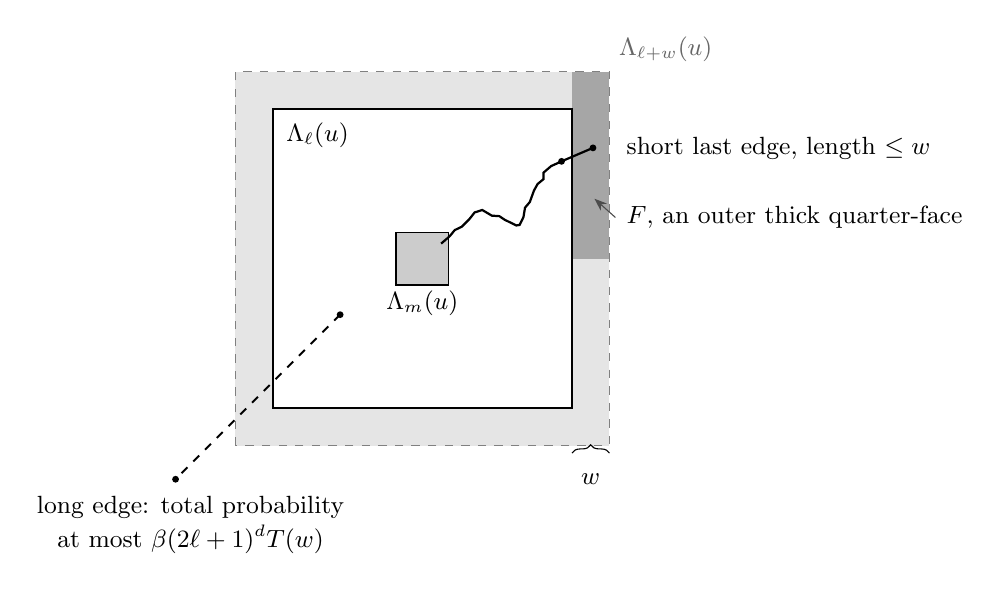
\begin{tikzpicture}[scale=0.95, >={Stealth[length=1.6mm]}]
  % shell
  \fill[black!10] (-2.5,-2.5) rectangle (2.5,2.5);
  \fill[white] (-2,-2) rectangle (2,2);
  % highlighted outer thick quarter-face
  \fill[black!35] (2,0) rectangle (2.5,2.5);
  \draw[line width=0.6pt] (-2,-2) rectangle (2,2);
  \draw[black!50, dashed] (-2.5,-2.5) rectangle (2.5,2.5);
  % seed box
  \draw[line width=0.6pt, fill=black!20] (-0.35,-0.35) rectangle (0.35,0.35);
  \node at (0,-0.6) {\small $\Lambda_m(u)$};
  % open path with a short last edge
  \draw[line width=0.8pt, decorate, decoration={random steps, segment length=3.2pt, amplitude=1.1pt}]
    (0.25,0.2) -- (0.8,0.65) -- (1.3,0.45) -- (1.62,1.15) -- (1.86,1.3);
  \draw[line width=0.8pt] (1.86,1.3) -- (2.28,1.48);
  \fill (1.86,1.3) circle (1.3pt); \fill (2.28,1.48) circle (1.3pt);
  \node[anchor=west] at (2.6,1.48) {\small short last edge, length $\le w$};
  \node[anchor=west] at (2.6,0.55) {\small $F$, an outer thick quarter-face};
  \draw[->, black!70] (2.58,0.55) -- (2.3,0.8);
  % long edge
  \fill (-1.1,-0.75) circle (1.3pt); \fill (-3.3,-2.95) circle (1.3pt);
  \draw[line width=0.7pt, dashed] (-1.1,-0.75) -- (-3.3,-2.95);
  \node[anchor=north, align=center] at (-3.1,-3.05) {\small long edge: total probability\\ \small at most $\beta(2\ell+1)^dT(w)$};
  % labels
  \node[anchor=north west] at (-1.95,1.95) {\small $\Lambda_\ell(u)$};
  \draw[decorate, decoration={brace, amplitude=3pt}] (2,-2.6) -- (2.5,-2.6) node[midway, below=2pt] {};
  \node at (2.25,-2.95) {\small $w$};
  \node[anchor=south west, black!60] at (2.5,2.5) {\small $\Lambda_{\ell+w}(u)$};
\end{tikzpicture}
\caption{Lemma~\ref{lem:faces} in a planar cross-section. An open path from $\Lambda_m(u)$ that
leaves $\Lambda_\ell(u)$ by an edge of length at most $w$ lands in the shell
$\Lambda_{\ell+w}(u)\setminus\Lambda_\ell(u)$ (light grey), which the $N_F$ outer thick quarter-faces
cover; one is shown in dark grey. A path can also leave by a long edge (dashed), which a
nearest-neighbour argument would not see; such edges are rare when $\ell^dT(w)$ is small.}
\label{fig:faces}
\end{figure}

\begin{lemma}[faces at a percolating parameter]\label{lem:faces}
Assume \textup{(Sym)} and $\theta(\beta)>0$. For $\ell>m$, $w\ge1$, every $u$ and every outer thick
quarter-face $F$ of $(u,\ell)$,
\[
\Pp_\beta\bigl(X(u,\ell,F)^c\bigr)\le\Bigl[\Pp_\beta(\Lam_m\text{ meets no infinite cluster})
+\beta(2\ell+1)^dT(w)\Bigr]^{1/N_F}.
\]
\end{lemma}
\begin{proof}
Take $u=0$. Let $E_{\mathrm{long}}$ be the event that some open edge $\{x,y\}$ has $x\in\Lam_\ell$
and $\norm{x-y}>w$; then
$\Pp(E_{\mathrm{long}})\le\sum_{x\in\Lam_\ell}\sum_{\norm{z}>w}(1-e^{-\beta J(z)})\le\beta(2\ell+1)^dT(w)$.
If $\Lam_m$ meets an infinite cluster, take a finite open path from $\Lam_m$ to a vertex outside
$\Lam_\ell$, and let $y$ be its first vertex outside $\Lam_\ell$ and $x$ its predecessor. Off
$E_{\mathrm{long}}$ we have $\norm{x-y}\le w$, so $y\in\Lam_{\ell+w}\setminus\Lam_\ell$. Choose $i$ with
$|y_i|>\ell$, $\sigma=\operatorname{sign}y_i$ and $\varepsilon_j=\operatorname{sign}y_j$ (either sign
if $y_j=0$); then $y\in F_{i,\sigma,\varepsilon}(0,\ell)$ and the path up to $y$ witnesses
$X(0,\ell,F_{i,\sigma,\varepsilon})$. Hence
$\Pp(\bigcap_FX(0,\ell,F)^c)\le\Pp(\Lam_m\text{ meets no infinite cluster})+\Pp(E_{\mathrm{long}})$.
The events $X(0,\ell,F)^c$ are decreasing and depend on finitely many bits. The signed coordinate
permutations fixing $0$ act transitively on the faces and, by (Sym), preserve the law, $\Lam_m$
and $\Lam_\ell$; so all $N_F$ complements have the same probability $a$. Harris's inequality gives
$a^{N_F}\le\Pp(\bigcap_FX(0,\ell,F)^c)$.
\end{proof}

\begin{lemma}[choice of scales]\label{lem:scales}
Assume \textup{(Sym)}, \textup{(Tail)} and $\theta(\beta)>0$. There are $f,\delta,\eta,\tau,\gamma\in(0,1)$,
positive integers $m,K,w,R,r$, constants $\rho_0,A,c_A,L>0$ and $q\in(\beta/2,\beta)$ such that:
\begin{enumerate}
\item[(S1)] $f<\frac12$ and $\sum_{n\ge1}2n3^n(2f)^{n/7}<1$;
\item[(S2)] $\delta+4(d+10)\eta/\delta<f$, $\tau<\eta/4$, $\gamma<\delta$ and $2\gamma/\tau<\eta/4$;
\item[(S3)] $\Pp_\beta(\Lam_m\text{ meets no infinite cluster})<\frac12(\gamma/2)^{N_F}$;
\item[(S4)] $\rho_0=\prod_e(1-e^{-(\beta/2)J(e)})$, the product over the pairs $e$ internal to $\Lam_m$ with $J(e)>0$;
$A=\beta\norm{J}_1$; $c_A=(1-e^{-A})/A$; $4/(K\rho_0)<\eta/4$; and $L=K(4m+3)^d/c_A$;
\item[(S5)] $\beta(41r+1)^dT(w)\le\min\{\frac12(\gamma/2)^{N_F},\eta/8\}$;
\item[(S6)] $w\ge m$, $R\ge m+w+8e^Lw/\eta$, $r>4(d+12)(R+w+1)$ and $r>m+w$;
\item[(S7)] for $\ell\in\cL:=\{2r,2r+1,10r-w\}$, every $u$ and every outer thick quarter-face $F$ of
$(u,\ell)$, $\Pp_q(X(u,\ell,F))>1-\gamma$.
\end{enumerate}
\end{lemma}
\begin{proof}
Choose $f$, then $\delta,\eta,\tau,\gamma$ in this order; then $m$ by~\eqref{eq:seed-infinite};
then $\rho_0,A,c_A,K,L$. None of these depends on $w$ or $r$. By (Tail) there are arbitrarily large
$w\ge m$ with $w^dT(w)$ as small as we like. For such $w$ put
$R=m+w+\lceil8e^Lw/\eta\rceil$ and $r=4(d+12)(R+w+2)$; then (S6) holds and $r\le C_0w$ with
$C_0$ depending only on $d,m,L,\eta$, so $\beta(41r+1)^dT(w)\le\beta(42C_0)^dw^dT(w)$ and (S5) holds
for a suitable such $w$. Every $\ell\in\cL$ satisfies $\ell>m$ and $2\ell+1\le41r+1$, so
Lemma~\ref{lem:faces}, (S3) and (S5) give $\Pp_\beta(X(u,\ell,F)^c)<\gamma/2$. These finitely many
events (up to translation) depend on finitely many bits whose probabilities are continuous in the
parameter, so (S7) holds for some $q\in(\beta/2,\beta)$.
\end{proof}

We fix these choices from now on, and write $\rho=\prod_e(1-e^{-qJ(e)})\ge\rho_0$ (over the same pairs) for the probability
that all pairs $e$ internal to a translate of $\Lam_m$ with $J(e)>0$ are open.

\section{Extension through a fresh region}\label{sec:extension}

\begin{figure}[tp]
\centering
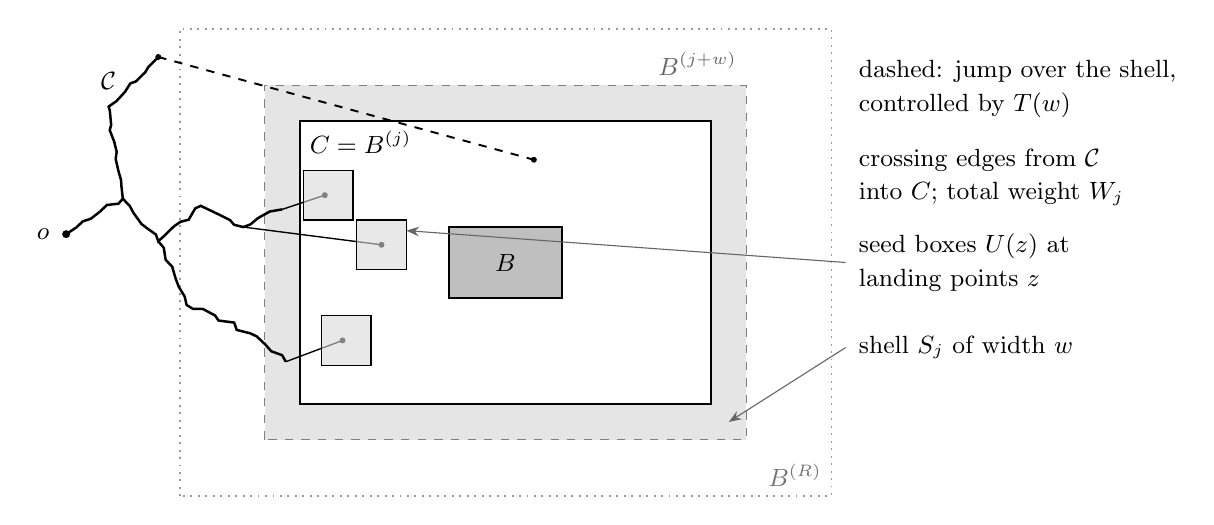
\begin{tikzpicture}[scale=0.9, >={Stealth[length=1.6mm]}]
  % B^(R) and D
  \draw[black!40, dotted, line width=0.7pt] (-4.6,-3.3) rectangle (4.6,3.3);
  \node[anchor=south east, black!55] at (4.6,-3.3) {\small $B^{(R)}$};
  % shell S_j between C and B^(j+w)
  \fill[black!10] (-3.4,-2.5) rectangle (3.4,2.5);
  \fill[white] (-2.9,-2.0) rectangle (2.9,2.0);
  \draw[line width=0.7pt] (-2.9,-2.0) rectangle (2.9,2.0);
  \draw[black!50, dashed] (-3.4,-2.5) rectangle (3.4,2.5);
  \node[anchor=north west] at (-2.9,2.0) {\small $C=B^{(j)}$};
  \node[anchor=south east, black!60] at (3.4,2.5) {\small $B^{(j+w)}$};
  % B
  \draw[line width=0.6pt, fill=black!25] (-0.8,-0.5) rectangle (0.8,0.5);
  \node at (0,0) {\small $B$};
  % outside cluster: path from o to shell, with branches
  \fill (-6.2,0.4) circle (1.6pt); \node[anchor=east] at (-6.3,0.4) {\small $o$};
  \draw[line width=0.9pt, decorate, decoration={random steps, segment length=3.5pt, amplitude=1.2pt}]
    (-6.2,0.4) -- (-5.4,0.9) -- (-4.9,0.3) -- (-4.3,0.8) -- (-3.7,0.5) -- (-3.15,0.75);
  \draw[line width=0.9pt, decorate, decoration={random steps, segment length=3.5pt, amplitude=1.2pt}]
    (-4.9,0.3) -- (-4.5,-0.6) -- (-3.6,-1.0) -- (-3.1,-1.4);
  \draw[line width=0.9pt, decorate, decoration={random steps, segment length=3.5pt, amplitude=1.2pt}]
    (-5.4,0.9) -- (-5.6,2.2) -- (-4.9,2.9);
  \node[anchor=south] at (-5.6,2.3) {\small $\mathcal C$};
  % crossing edges and landing points with seed boxes
  \foreach \a/\b/\c/\e in {-3.15/0.75/-2.55/0.95, -3.1/-1.4/-2.3/-1.1, -3.7/0.5/-1.75/0.25}{
     \draw[line width=0.5pt] (\a,\b) -- (\c,\e);
     \fill (\c,\e) circle (1.2pt);
  }
  \draw[line width=0.5pt, fill=black!15, fill opacity=0.6] (-2.85,0.6) rectangle (-2.15,1.3);
  \draw[line width=0.5pt, fill=black!15, fill opacity=0.6] (-2.6,-1.45) rectangle (-1.9,-0.75);
  \draw[line width=0.5pt, fill=black!15, fill opacity=0.6] (-2.1,-0.1) rectangle (-1.4,0.6);
  % long jump over the shell
  \fill (-4.9,2.9) circle (1.2pt);
  \draw[line width=0.7pt, dashed] (-4.9,2.9) -- (0.4,1.45);
  \fill (0.4,1.45) circle (1.2pt);
  % annotations
  \node[anchor=west, align=left] at (4.85,1.2) {\small crossing edges from $\mathcal C$\\ \small into $C$; total weight $W_j$};
  \node[anchor=west, align=left] at (4.85,0.0) {\small seed boxes $U(z)$ at\\ \small landing points $z$};
  \node[anchor=west, align=left] at (4.85,-1.2) {\small shell $S_j$ of width $w$};
  \node[anchor=west, align=left] at (4.85,2.45) {\small dashed: jump over the shell,\\ \small controlled by $T(w)$};
  \draw[->, black!60] (4.8,-1.2) -- (3.15,-2.25);
  \draw[->, black!60] (4.8,0.0) -- (-1.4,0.45);
\end{tikzpicture}
\caption{The extension lemma (Lemma~\ref{lem:extension}) in a planar cross-section. The cluster
$\mathcal C$ of $o$ outside $C=B^{(j)}$ reaches the shell $S_j$. All crossing edges from
$\mathcal C$ into $C$ are closed with probability exactly $e^{-W_j}$, which is cheap when $W_j$ is
small; when $W_j$ is large, the landing points $z$ in one residue class carry disjoint seed boxes
$U(z)$, which give many independent chances to reach a good relay centre. Entrances that jump over
the shell are rare by the tail condition.}
\label{fig:extension}
\end{figure}

\begin{lemma}[extension]\label{lem:extension}
Let $G=(V,E)$ be a finite graph as in Section~\ref{sec:prelim}, $D\subset V$ a rectangle with
$|D|\le(41r+1)^d$ and $(F_q(D))$, $B$ a rectangle with $B^{(R)}\subset D$, $o\in V\setminus B^{(R)}$
and $T\subset V$. Assume:
\begin{enumerate}
\item[(E2)] every edge $\{x,z\}$ of $G$ with $z\in B^{(R)}$ and $x\notin D$ has $\lambda_{xz}\le qJ(x-z)$;
\item[(E3)] for every $u\in B^{(R)}$ there are $\ell\in\cL$ and an outer thick quarter-face $F$ of $(u,\ell)$
with $\Lam_{\ell+w}(u)\subset D$ and $F\subset T$.
\end{enumerate}
Then $\Pp(o\lr B,\ o\nlr T)<\eta$.
\end{lemma}

\begin{proof}
By $(F_q(D))$ and (E2), every edge $\{x,z\}$ with $z\in B^{(R)}$ and $x\notin B^{(R)}$ has
$\lambda_{xz}\le qJ(x-z)$; hence $\sum_x\lambda_{xz}\le q\norm{J}_1\le A$ for $z\in B^{(R)}$.

\emph{Step 1: a layer.} For an integer $j\in[m,R)$ let $\zeta_j$ be the bits internal to
$V\setminus B^{(j)}$, let $\cC_j$ be the open cluster of $o$ in the graph on $V\setminus B^{(j)}$ with
these bits, and set
\[
W_j=\sum_{x\in\cC_j}\sum_{z\in B^{(j)}}\lambda_{xz},\qquad S_j=B^{(j+w)}\setminus B^{(j)},
\]
\[
L_j=\{W_j<L,\ \cC_j\cap S_j\ne\varnothing\},\qquad
\mathrm{Cl}_j=\{\text{every edge between }\cC_j\text{ and }B^{(j)}\text{ is closed}\}.
\]
Here $W_j\le|B^{(j)}|A<\infty$. The crossing bits between $V\setminus B^{(j)}$ and $B^{(j)}$ are
independent of $\zeta_j$, so $\Pp(\mathrm{Cl}_j\mid\zeta_j)=e^{-W_j}\ge e^{-L}$ on $L_j$. On
$\mathrm{Cl}_j$ the open cluster $C(o)$ of $o$ in $G$ equals $\cC_j$, because every other edge
leaving $\cC_j$ is internal to $V\setminus B^{(j)}$ and therefore closed by maximality.

Let $\cJ=\{m+kw:k\ge0\}\cap[m,R)$. If $j'<j$ both lie in $\cJ$, then $j'+w\le j$; on
$L_j\cap\mathrm{Cl}_j$ we have $C(o)=\cC_j\subset V\setminus B^{(j)}$, hence $\cC_{j'}=C(o)$, while
$S_{j'}\subset B^{(j)}$, so $\cC_{j'}\cap S_{j'}=\varnothing$ and $L_{j'}$ fails. The events
$L_j\cap\mathrm{Cl}_j$, $j\in\cJ$, are therefore pairwise disjoint, and
\[
e^{-L}\sum_{j\in\cJ}\Pp(L_j)\le\sum_{j\in\cJ}\Pp(L_j\cap\mathrm{Cl}_j)\le1.
\]
Since $|\cJ|\ge(R-m)/w$, we can fix $j\in\cJ$ with $\Pp(L_j)\le e^Lw/(R-m)\le\eta/8$, by (S6).

Let $E_{\mathrm{long}}$ be the event that some open edge $\{x,z\}$ has $z\in B^{(R)}$ and
$\norm{x-z}>w$. Then
$\Pp(E_{\mathrm{long}})\le\sum_{z\in B^{(R)}}\sum_{\norm{x-z}>w}\lambda_{xz}\le q|D|T(w)\le\eta/8$
by (S5). If $o\lr B$, $W_j<L$ and $\cC_j\cap S_j=\varnothing$, then an open path from $o$ enters
$B^{(j)}$ for the first time at some $z$ from a predecessor $x\in\cC_j\setminus B^{(j+w)}$, so
$\norm{x-z}>w$ and $E_{\mathrm{long}}$ occurs. Hence
\begin{equation}\label{eq:low-weight}
\Pp(o\lr B,\ W_j<L)\le\Pp(L_j)+\Pp(E_{\mathrm{long}})\le\eta/4.
\end{equation}

\emph{Step 2: relay quality.} Put $C=B^{(j)}$ and let $\xi$ be the bits internal to $C$. Every side
of $C$ has at least $2j+1\ge2m+1$ points. For $z\in C$ let $v(z)$ be obtained from $z$ by clamping
each coordinate to the corresponding side of $C$ shrunk by $m$ at both ends, let
$U(z)=\Lam_m(v(z))\subset C$ (so $z\in U(z)$), let $O(z)$ be the event that all bits internal to
$U(z)$ are open, so $\Pp(O(z))=\rho$, and put
\[
g(z)=\Pp(v(z)\lr T\mid\xi),\qquad A_\xi=\{v(z):z\in C,\ g(z)>1-\tau\}.
\]
$A_\xi$ is a function of $\xi$. Fix $z$. By (E3) at $u=v(z)\in B^{(R)}$ there are $\ell\in\cL$ and $F$
with $\Lam_{\ell+w}(v(z))\subset D$ and $F\subset T$; the event $X(v(z),\ell,F)$ uses only bits
internal to $D$, so by $(F_q(D))$ and (S7) its probability exceeds $1-\gamma$. By (Pos) and (Sym)
an open box is connected through its nearest-neighbour pairs, so on $O(z)\cap X(v(z),\ell,F)$ we
have $v(z)\lr T$. Harris's inequality gives $\Pp(O(z),\ v(z)\nlr T)\le\rho\gamma$, and since $O(z)$
is $\xi$-measurable,
\begin{equation}\label{eq:relay-quality}
\tau\,\Pp\bigl(O(z),\ g(z)\le1-\tau\bigr)\le\E\bigl[\1_{O(z)}(1-g(z))\bigr]=\Pp\bigl(O(z),\ v(z)\nlr T\bigr)\le\rho\gamma.
\end{equation}

\emph{Step 3: entrances.} Condition on $\zeta=\zeta_j$; write $\cC=\cC_j$ and
$a_z=\sum_{x\in\cC}\lambda_{xz}$ for $z\in C$, so that $W_j=\sum_{z\in C}a_z$ and $a_z\le A$. Among the
$(4m+3)^d$ residue classes of $C$ modulo $4m+3$, choose (as a function of $\zeta$) a class $Z$ with
$\sum_{z\in Z}a_z\ge W_j/(4m+3)^d$. Distinct $z,z'\in Z$ satisfy $\norm{z-z'}\ge4m+3$, and clamping
moves each coordinate by at most $m$, so $\norm{v(z)-v(z')}\ge2m+3$ and the boxes $U(z)$, $z\in Z$,
are disjoint.

Let $\Sigma_z$ be the event that some edge between $\cC$ and $z$ is open and $O(z)$ holds. Given
$\zeta$, the crossing bits are independent of $\xi$, edges into distinct $z$ are distinct, and the
events $O(z)$, $z\in Z$, use disjoint bits of $\xi$; hence the events $\Sigma_z$, $z\in Z$, are
independent with $\Pp(\Sigma_z\mid\zeta)=\rho(1-e^{-a_z})$. Let $S=\sum_{z\in Z}\1_{\Sigma_z}$ and
$\mu=\sum_{z\in Z}(1-e^{-a_z})$. Since $a\mapsto(1-e^{-a})/a$ is decreasing, $1-e^{-a_z}\ge c_Aa_z$
and $\mu\ge c_AW_j/(4m+3)^d$, which is at least $K$ on $\{W_j\ge L\}$. By Chebyshev's inequality,
on $\{W_j\ge L\}$,
\[
\Pp(S<\rho\mu/2\mid\zeta)\le\frac{4}{\rho\mu}\le\frac4{\rho_0K}<\frac\eta4 .
\]
Let $Z_{\mathrm{bad}}=\sum_{z\in Z}\1_{\Sigma_z}\1\{g(z)\le1-\tau\}$. By the independence of the
crossing bits from $\xi$ and~\eqref{eq:relay-quality},
$\E[Z_{\mathrm{bad}}\mid\zeta]=\sum_z(1-e^{-a_z})\Pp(O(z),g(z)\le1-\tau)\le\mu\rho\gamma/\tau$, so
$\Pp(Z_{\mathrm{bad}}\ge\rho\mu/2\mid\zeta)\le2\gamma/\tau<\eta/4$. If $S\ge\rho\mu/2>Z_{\mathrm{bad}}$,
some $z\in Z$ has $\Sigma_z$ and $g(z)>1-\tau$: then $o$ reaches some $x\in\cC$, the open edge
$\{x,z\}$, and $v(z)\in A_\xi$ through the open box $U(z)$. Together with~\eqref{eq:low-weight},
\[
\Pp(o\lr B,\ o\nlr A_\xi)\le\tfrac34\eta .
\]

\emph{Step 4: the target.} Condition on $\xi$. Then $A_\xi$ is fixed, the remaining bits keep their
product law, and $\Pp(a\lr T\mid\xi)>1-\tau$ for every $a\in A_\xi$. Corollary~\ref{cor:failure},
applied with the bits of $\xi$ fixed, gives $\Pp(o\lr A_\xi,\ o\nlr T\mid\xi)\le\tau<\eta/4$.
Splitting according to whether $o\lr A_\xi$ gives $\Pp(o\lr B,\ o\nlr T)<\eta$.
\end{proof}

\section{Relay between neighbouring coarse cubes}\label{sec:relay}

For $v=(v_1,v_2)\in\Z^2$ let
\[
c_v=(20r+1)(v_1,v_2,0,\dots,0)\in\Z^d,\qquad Q_v=\Lam_{10r}(c_v),\qquad B_v=\Lam_{4r}(c_v).
\]
The cubes $Q_v$ are vertex-disjoint. For neighbours $v,x$ in $\Z^2$, let $I_{vx}$ be the finite set
of pairs $\{y,y'\}$ with $y\in Q_v$, $y'\in Q_x$ and $J(y-y')>0$. The union $D_{vx}=Q_v\cup Q_x$ is a
rectangle with $|D_{vx}|=(40r+2)(20r+1)^{d-1}\le(41r+1)^d$, whose internal bits are those internal to
$Q_v$, those internal to $Q_x$, and $I_{vx}$. Let $D^\circ_{vx}$ be the set of points of $D_{vx}$ at
distance more than $2r$ from $\Z^d\setminus D_{vx}$.

\begin{lemma}[relay]\label{lem:relay}
Let $v,x$ be neighbours in $\Z^2$ and $G$ a finite graph as in Section~\ref{sec:prelim} with
$D=D_{vx}\subset V$ and $(F_q(D))$. Assume
\begin{enumerate}
\item[(E2$^\circ$)] every edge $\{y,z\}$ of $G$ with $z\in D^\circ_{vx}$ and $y\notin D$ has
$\lambda_{yz}\le qJ(y-z)$.
\end{enumerate}
If $o\in V\setminus D$, then $\Pp(o\lr B_v,\ o\nlr B_x)\le(d+10)\eta$.
\end{lemma}

\begin{proof}
By (Sym) we may assume $c_v=0$ and $c_x=(20r+1)e_1$, so that
$D=[-10r,30r+1]\times[-10r,10r]^{d-1}$. Put $R'=R+w$. We define rectangles $P_0,\dots,P_{d+10}$ and
apply Lemma~\ref{lem:extension} with $B=P_{k-1}$ and $T=P_k$; the radius is $2r$ for $k\le d+9$
and $2r+1$ for $k=d+10$. Let $P_0=B_v$. For $t=1,\dots,d$ let $P_t$ be centred at $0$ with
half-width $2r+tR'$ in directions $h\le t$ and $4r+tR'$ in directions $h>t$. For $i=1,\dots,10$
put $s_i=2r$ ($i\le9$), $s_{10}=2r+1$, $z_i=(s_1+\dots+s_i)e_1$, $w_i=2r+(d+i)R'$, and
$P_{d+i}=\Lam_{w_i}(z_i)$.

\emph{Contraction steps.} Let $1\le t\le d$ and $u\in P_{t-1}^{(R)}$. Then $|u_h|\le2r+tR'-w$ for
$h<t$ and $|u_h|\le4r+tR'-w$ for $h\ge t$. Take $F=F_{t,\sigma,\varepsilon}(u,2r)$ with
$\sigma=-\operatorname{sign}u_t$ and $\varepsilon_j=-\operatorname{sign}u_j$ (with
$\operatorname{sign}0=+1$). A point $y\in F$ has $y_t=u_t+\sigma s$ with $s\in(2r,2r+w]$, so
$|y_t|\le|u_t|-2r\le2r+tR'$ if $|u_t|\ge2r+w$ and $|y_t|\le2r+w$ otherwise. For $j\ne t$, $y_j$ lies
between $u_j$ and $u_j-\operatorname{sign}(u_j)(2r+w)$, so $|y_j|\le\max\{|u_j|,2r+w\}$, which is at
most the half-width of $P_t$ in direction $j$. Thus $F\subset P_t$. The coordinates of
$\Lam_{2r+w}(u)$ are at most $6r+dR'+w<8r$ in absolute value, by (S6), so $\Lam_{2r+w}(u)\subset Q_v$
and $P_{t-1}^{(R)}\subset D^\circ_{vx}$. After the last contraction, $P_d=\Lam_{2r+dR'}(0)$.

\emph{Translation steps.} Let $1\le i\le10$ and $u\in P_{d+i-1}^{(R)}$, so
$\norm{u-z_{i-1}}\le w_{i-1}+R$ with $w_0=2r+dR'$. Take $F=F_{1,+,\varepsilon}(u,s_i)$ with
$\varepsilon_j=-\operatorname{sign}u_j$. For $y\in F$,
$y_1-(z_i)_1=(u_1-(z_{i-1})_1)+(y_1-u_1-s_i)$ with $y_1-u_1-s_i\in(0,w]$, so
$|y_1-(z_i)_1|\le w_{i-1}+R+w=w_i$, and $|y_j|\le\max\{|u_j|,s_i+w\}\le w_i$ for $j\ge2$. Thus
$F\subset P_{d+i}$. The first coordinates of $\Lam_{s_i+w}(u)$ lie in
$[-4r-(d+11)R'-1,\ 22r+(d+11)R'+1]$ and the others have absolute value at most $4r+(d+11)R'+1$; by
(S6) these lie in $D$ at distance more than $2r$ from its complement. Finally $z_{10}=c_x$ and
$w_{10}=2r+(d+10)R'<4r$, so $P_{d+10}\subset B_x$.

Each $P_{k-1}^{(R)}$ lies in $D^\circ_{vx}$, so (E2$^\circ$) gives (E2), and (E3) was just verified; also
$o\notin D$. If $o\lr P_0$ but $o\nlr P_{d+10}$, then $o\lr P_{k-1}$ and $o\nlr P_k$ for some $k$, and
the union bound over the $d+10$ applications of Lemma~\ref{lem:extension} proves the claim.
\end{proof}

\section{Exploration and the proof of Theorem~\ref{thm:main}}\label{sec:exploration}

We follow the exploration of~\cite[\S6]{OpenAIZ3}, with the long-range interfaces $I_{vx}$. Let
$o=0\in Q_0$, and let $\cI$ be the event that all bits internal to $Q_0$ are open. It prescribes
finitely many bits, each of probability in $(0,1)$, so $\Pp_q(\cI)>0$, and under
$\Pp_\cI=\Pp_q(\cdot\mid\cI)$ all other bits are independent with their parameter-$q$ law.

\paragraph{The exploration.} The coarse root $0\in\Z^2$ is declared good and visited, but is never queued
or processed; its four neighbours are put in a queue with parent $0$. A coarse vertex is \emph{visited} once it has been
queued, and \emph{pending} until it is processed; vertices are processed in queue order, and none is queued
twice. For a pending $v$, let $G(v)$ be the graph consisting of the cubes on the parent chain of
$v$ back to the root, the bits internal to these cubes, and the interfaces $I$ between successive
cubes of the chain, and no other pairs. Put $H_v=\{o\lr B_v\text{ in }G(v)\}$. To process $v$, reveal
the bits internal to $Q_v$ and those of $I_{pv}$, where $p$ is the parent of $v$. For each unvisited
neighbour $x$ of $v$, let $G'=G(v)\cup Q_x\cup I_{vx}$ (with the bits internal to $Q_x$) and compute
\[
b_x=\Pp_\cI(o\lr B_x\text{ in }G'\mid\text{history after this reveal}),
\]
which reveals nothing. Declare $v$ \emph{good} if $H_v$ holds and $b_x>1-\delta$ for every such $x$,
and in that case queue these $x$ with parent $v$; otherwise declare $v$ \emph{bad}. We maintain
\begin{equation}\label{eq:promise}
\Pp_\cI(H_v\mid\text{revealed history})>1-\delta\qquad\text{for every pending }v.
\end{equation}

\begin{lemma}[freshness and the initial promise]\label{lem:fresh}
Conditional on any revealed history of positive probability, the bits that are neither prescribed
by $\cI$ nor revealed are independent with their parameter-$q$ law, and~\eqref{eq:promise} holds at
every step.
\end{lemma}
\begin{proof}
Each step reveals a finite set of bits determined by earlier revealed values, and all decisions are
functions of revealed values; induction gives the first claim. The unknown bits of $H_x$ for a
pending $x$ with parent $v$ are internal to $Q_x$ or lie in $I_{vx}$. The cubes are vertex-disjoint,
each step reveals the internal bits of one cube and its own parent interface, and $G(x)$ contains no
other pairs, so these bits stay unrevealed while $x$ is pending; together with the definition of
\emph{good}, this keeps~\eqref{eq:promise} for every queued $x$ once it holds when $x$ is queued.

It remains to check~\eqref{eq:promise} for the root's neighbours. Let $v$ be one; by symmetry $Q_0$
lies in direction $-e_1$ from $Q_v$. Let $\ell'=10r-w\in\cL$, $u=c_v-we_1$ and
$F=F_{1,-,(+,\dots,+)}(u,\ell')$. Then $\Lam_{\ell'}(u)\subset Q_v$; $\Lam_m(u)\subset B_v$ since
$m+w\le4r$; and $F\subset Q_0$, since its first coordinates lie in $[(c_v)_1-10r-w,(c_v)_1-10r-1]$
and its other coordinates in $[0,10r]$. On $X(u,\ell',F)$, the box $\Lam_m(u)$ is joined inside $Q_v$
to a vertex with an open edge of length at most $w$ into $Q_0$, and this edge lies in $I_{0v}$, so
$X(u,\ell',F)\cap\cI\subset H_v$ (the cube $Q_0$ is open and connected by (Pos)). The event
$X(u,\ell',F)$ depends only on bits internal to $Q_v$ and on pairs of $I_{0v}$, which are independent
of $\cI$; hence $\Pp_\cI(H_v)\ge\Pp_q(X(u,\ell',F))>1-\gamma>1-\delta$ by (S7) and (S2).
\end{proof}

\begin{lemma}\label{lem:bad}
Immediately before a pending $v$ is processed, the conditional probability that $v$ is declared bad
is less than $f$.
\end{lemma}
\begin{proof}
Fix an unvisited neighbour $x$ of $v$ and let $D=D_{vx}$. Neither $v$ (pending) nor $x$ (unvisited)
has been processed and $I_{vx}$ is not a parent interface yet, so every bit internal to $D$ is fresh
with parameter $q$, and $(F_q(D))$ holds in $G'$. The pairs of $G'$ with one endpoint in $D$ and the
other outside are those of $I_{pv}$, which is still unrevealed, with $\lambda=qJ$; so (E2$^\circ$)
holds. Since $o\notin D$, Lemma~\ref{lem:relay} gives
$\Pp_\cI(H_v\cap\{o\nlr B_x\text{ in }G'\}\mid\text{history})\le(d+10)\eta$, and the tower property
gives $\Pp_\cI(H_v,\ b_x\le1-\delta\mid\text{history})\le(d+10)\eta/\delta$. With at most four such
$x$ and~\eqref{eq:promise}, $\Pp_\cI(v\text{ bad}\mid\text{history})\le\delta+4(d+10)\eta/\delta<f$
by (S2).
\end{proof}

\begin{lemma}\label{lem:badset}
For every deterministic set of $k$ distinct coarse vertices, the $\Pp_\cI$-probability that all of
them are processed and declared bad is at most $f^k$.
\end{lemma}
\begin{proof}
The root is good, so assume it is not in the set $S$. Let $\tau_j$ be the time at which the $j$th
member of $S$ is processed ($\tau_j=\infty$ if there is none) and $E_j$ the event that $\tau_j<\infty$
and the first $j$ processed members are bad. For each finite $t$ the event
$\{\tau_j=t\}\cap E_{j-1}$ is determined before the reveal at time $t$, so Lemma~\ref{lem:bad} gives
$\Pp_\cI(E_j)\le f\sum_t\Pp_\cI(\tau_j=t,E_{j-1})\le f\,\Pp_\cI(E_{j-1})$, and induction finishes the proof.
\end{proof}

\begin{proof}[Proof of Theorem~\ref{thm:main}]
By Lemma~\ref{lem:basic}, $0<\beta_c<\infty$. Suppose that $\theta(\beta_c)>0$ and choose the
parameters of Lemma~\ref{lem:scales} with $\beta=\beta_c$. Let $X\subset\Z^2$ be the set of good coarse
vertices. If $X$ is finite, the queue empties after finitely many steps, and every coarse vertex
outside $X$ adjacent to $X$ has been processed and declared bad. Apply Lemma~\ref{lem:contours} to
$X$: its boundary contains a cycle of some length $n$ from a family of at most $2n3^n$ candidates,
each with $k\ge n/7$ crossed edges with disjoint endpoints, each of which has a bad endpoint outside
$X$. Choosing one endpoint per edge in $2^k$ ways, Lemma~\ref{lem:badset} bounds the probability of a
given candidate by $(2f)^k\le(2f)^{n/7}$. By (S1),
$\Pp_\cI(|X|<\infty)\le\sum_n2n3^n(2f)^{n/7}<1$. Every good non-root vertex $v$ satisfies $H_v$, and
the boxes $B_v$ are disjoint, so with positive $\Pp_\cI$-probability the open cluster of $o$ in the
long-range model is infinite. Hence $\theta(q)\ge\Pp_q(\cI)\Pp_\cI(|X|=\infty)>0$ with $q<\beta_c$,
a contradiction.
\end{proof}

\section{The corollaries, and where the hypotheses enter}\label{sec:corollaries}

\begin{proof}[Proof of Corollary~\ref{cor:power}]
If $\alpha>d$ then $T(n)\le C'n^{-\alpha}$, so (Tail) holds, and (Pos) holds by the lower bound;
apply Theorem~\ref{thm:main}. If $\alpha<d$, put $s=d+\alpha<2d$ and $P_k=1-e^{-\beta J(k)}$ at a
parameter $\beta$ with $\theta(\beta)>0$. Berger's theorem~\cite[Theorem~2.6]{Berger2002} states: if
$\{P_k\}$ is percolating and $\liminf_{\norm{k}\to\infty}P_k\norm{k}_1^{s}>0$ for some $s<2d$, then
$\{(1-\epsilon)P_k\}$ is percolating for some $\epsilon>0$ (his standing assumption is
$0\le P_k=P_{-k}<1$, which holds here). Monotonicity and $1-e^{-t}\ge t/2$ on $[0,1]$ give
$P_k\ge(\beta c/2)\norm{k}^{-s}\ge(\beta c/2)\norm{k}_1^{-s}$ for large $\norm{k}$. Concavity of
$t\mapsto1-e^{-t}$ gives $1-e^{-(1-\epsilon)\beta J}\ge(1-\epsilon)(1-e^{-\beta J})$, so
$\theta((1-\epsilon)\beta)>0$. Thus $\theta(\beta)>0$ forces $\beta>\beta_c$.
\end{proof}

\begin{proof}[Proof of Corollary~\ref{cor:exp}]
Exponential decay and finite range both give $n^dT(n)\to0$.
\end{proof}

\begin{remark}[where the hypotheses enter]\label{rem:hyp}
The tail condition is used only in (S5), at one pair of scales $(w,r)$ with $r$ a large constant
multiple of $w$ fixed by (S6): in
Lemma~\ref{lem:faces}, for exits from $\Lam_\ell$ by edges longer than $w$, and in the event
$E_{\mathrm{long}}$ of Lemma~\ref{lem:extension}, for entrances that jump over the shell. The layer
argument needs $R\gg e^Lw$ and the relay needs $r\gg R+w$; both hold with $r\le C_0w$, and
(Tail) then makes $\beta(41r+1)^dT(w)\le\beta(42C_0)^dw^dT(w)$ small. Summability gives the uniform bound $a_z\le A$, which turns a large crossing
weight into many seed attempts. (Sym) gives the equal probabilities of the faces in
Lemma~\ref{lem:faces} and the orientation reductions. (Pos) gives $\beta_c<\infty$ and the
connectivity of open boxes. The dimension $d\ge2$ enters through the coordinate plane in
Lemma~\ref{lem:basic} and the coarse lattice $\Z^2$ with its contour count.
\end{remark}

\begin{remark}[the borderline]\label{rem:border}
For $J(x)\asymp\norm{x}^{-2d}$ the quantity $n^dT(n)$ stays bounded away from zero, and nothing in the
argument guarantees (S5) and (S6) together: long edges at scale $n$ leave the cube $[-n,n]^d$ with
probability of order one at every scale. In $d=1$ and $J(x)\asymp|x|^{-2}$ the transition is discontinuous
\cite{AizenmanNewman1986,DuminilCopinGarbanTassion2020}, and the argument above also lacks the coarse
plane. Apart from sufficiently spread-out kernels in $d\ge7$, where $d>6=3(\alpha\wedge2)$
and~\cite{HeydenreichHofstadSakai2008} applies, whether $\theta(\beta_c)=0$ for $\alpha=d\ge2$ remains open.
\end{remark}

{\small\raggedright
\begin{thebibliography}{99}

\bibitem{AizenmanNewman1986}
M.~Aizenman and C.~M. Newman.
\newblock Discontinuity of the percolation density in one-dimensional $1/|x-y|^2$ percolation models.
\newblock {\em Comm. Math. Phys.}, 107(4):611--647, 1986.

\bibitem{AngelEtAl2026}
O.~Angel, D.~de~la Riva, C.~Panagiotis, and Y.~Shi.
\newblock Continuity of the phase transition for long-range {B}ernoulli percolation with exponential decay on $\mathbb{Z}^2$.
\newblock Preprint, arXiv:2610.35233, 2026.

\bibitem{Berger2002}
N.~Berger.
\newblock Transience, recurrence and critical behavior for long-range percolation.
\newblock {\em Comm. Math. Phys.}, 226:531--558, 2002.
\newblock \href{https://doi.org/10.1007/s002200200617}{doi:10.1007/s002200200617}, arXiv:math/0110296.

\bibitem{BlancRenaudie2026}
A.~Blanc-Renaudie.
\newblock Notes on {K}ozma and {N}itzan's proof of $\theta(p_c)=0$.
\newblock Preprint, arXiv:2610.10502, 2026.

\bibitem{DuminilCopinGarbanTassion2020}
H.~Duminil-Copin, C.~Garban, and V.~Tassion.
\newblock Long-range models in 1{D} revisited.
\newblock Preprint, arXiv:2011.04642, 2020.

\bibitem{DuminilCopinSidoraviciusTassion2016}
H.~Duminil-Copin, V.~Sidoravicius, and V.~Tassion.
\newblock Absence of infinite cluster for critical {B}ernoulli percolation on slabs.
\newblock {\em Comm. Pure Appl. Math.}, 69(7):1397--1411, 2016.

\bibitem{FitznerHofstad2017}
R.~Fitzner and R.~van~der Hofstad.
\newblock Mean-field behavior for nearest-neighbor percolation in $d>10$.
\newblock {\em Electron. J. Probab.}, 22:43, 2017.
\newblock \href{https://doi.org/10.1214/17-EJP56}{doi:10.1214/17-EJP56}.

\bibitem{Gouere2026}
J.-B. Gou{\'e}r{\'e}.
\newblock On the proof of the {K}ozma--{N}itzan conjecture.
\newblock Preprint, arXiv:2610.30063, 2026.

\bibitem{GrimmettMarstrand1990}
G.~R. Grimmett and J.~M. Marstrand.
\newblock The supercritical phase of percolation is well behaved.
\newblock {\em Proc. Roy. Soc. London Ser. A}, 430(1879):439--457, 1990.

\bibitem{HaraSlade1990}
T.~Hara and G.~Slade.
\newblock Mean-field critical behaviour for percolation in high dimensions.
\newblock {\em Comm. Math. Phys.}, 128(2):333--391, 1990.

\bibitem{Harris1960}
T.~E. Harris.
\newblock A lower bound for the critical probability in a certain percolation process.
\newblock {\em Proc. Cambridge Philos. Soc.}, 56:13--20, 1960.

\bibitem{HeydenreichHofstadSakai2008}
M.~Heydenreich, R.~van~der Hofstad, and A.~Sakai.
\newblock Mean-field behavior for long- and finite range {I}sing model, percolation and self-avoiding walk.
\newblock {\em J. Stat. Phys.}, 132:1001--1049, 2008.
\newblock \href{https://doi.org/10.1007/s10955-008-9580-5}{doi:10.1007/s10955-008-9580-5}.

\bibitem{Hutchcroft2021}
T.~Hutchcroft.
\newblock Power-law bounds for critical long-range percolation below the upper-critical dimension.
\newblock {\em Probab. Theory Related Fields}, 181:533--570, 2021.
\newblock arXiv:2008.11197.

\bibitem{Kesten1980}
H.~Kesten.
\newblock The critical probability of bond percolation on the square lattice equals $1/2$.
\newblock {\em Comm. Math. Phys.}, 74:41--59, 1980.

\bibitem{KozmaNitzan2024}
G.~Kozma and S.~Nitzan.
\newblock A reduction of the $\theta(p_c)=0$ problem to a conjectured inequality.
\newblock Preprint, arXiv:2401.12397, 2024.

\bibitem{Leder2026}
J.~Leder.
\newblock $\theta(p_c)=0$ for {B}ernoulli bond percolation on $\mathbb{Z}^d$ in all dimensions $d\ge2$, in {L}ean~4/{M}athlib, 2026.
\newblock \url{https://github.com/anthropics/formal-math/tree/795efb86f191735c5481675763537cfb4ff37e55/percolation}.

\bibitem{OpenAIZ3}
OpenAI.
\newblock Critical bond and site percolation on the cubic lattice, 2026.
\newblock \url{https://github.com/openai/math/tree/adc7f1241b42e322a6451854ab7e4b4c146bf78a/preprints/Critical-bond-and-site-percolation-on-the-cubic-lattice-September-24-2026}.

\bibitem{OpenAIQT}
OpenAI.
\newblock No percolation at criticality on quasi-transitive graphs, 2026.
\newblock \url{https://github.com/openai/math/tree/adc7f1241b42e322a6451854ab7e4b4c146bf78a/preprints/No-percolation-at-criticality-on-quasi-transitive-graphs-September-24-2026}.

\bibitem{PeiLean}
Y.~R.~Pei.
\newblock Lean~4 formalization of Theorem~1.1, 2026.
\newblock \url{https://github.com/PeaBrane/lr-continuity-lean}.

\end{thebibliography}
}

\end{document}
